\paragraph{API Umbrella}
\label{soa:tecnologias:api-umbrella}

Es un producto open source desarrollado por la NREL (\eng{National Renewable Energy Laboratory}) que actualmente está en uso por el Gobierno de Estados Unidos en la \gls{acro:api} su sitio de \eng{open data}. Su función es la de un proxy que se ubica delante de las aplicaciones que proveen las \glspl{acro:api} (los \eng{\gls{acro:api} backends}) y procesa los requerimientos entrantes para esos servicios con un conjunto de reglas configurables, envía esos requerimientos a los proveedores correspondientes para finalmente enviar al cliente la respuesta. En la superficie es similar a Kong, pero su arquitectura interna es mucho más compleja, como veremos en breve.

\subparagraph{Licencia}

Este producto está publicado bajo licencia MIT\footnote{\url{https://github.com/NREL/api-umbrella/blob/master/LICENSE.txt}}.

\subparagraph{Arquitectura interna}

\begin{figure}
  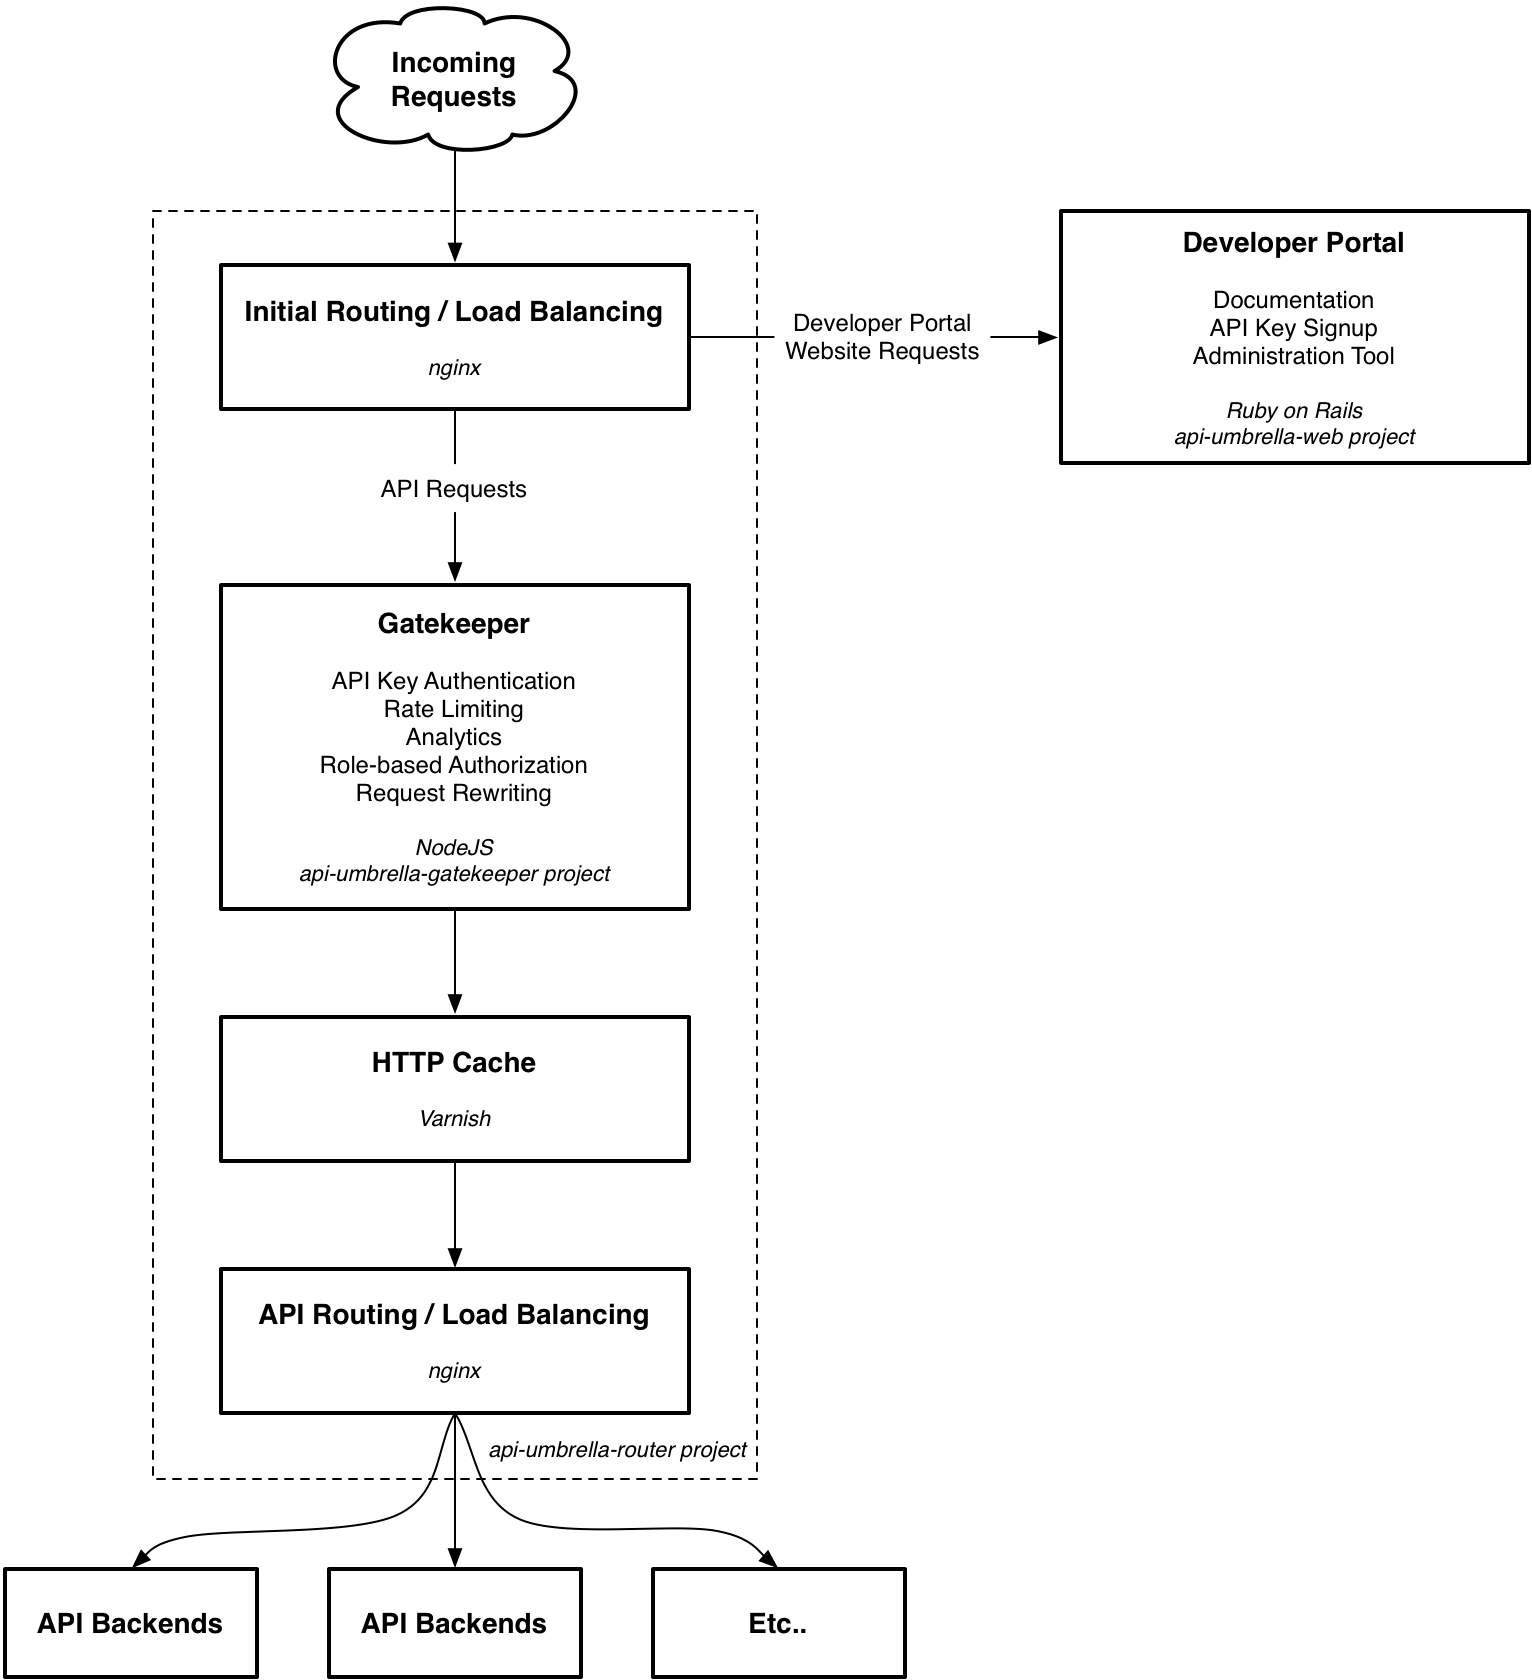
\includegraphics[width=\linewidth]{src/images/03-capitulo-3/tecnologias/api-umbrella/api-umbrella-arq.png}
  \caption{Arquitectura interna de API Umbrella}
  \label{fig:arquitectura-interna-api-umbrella}
\end{figure}

Como se puede ver en el diagrama \nameref{fig:arquitectura-interna-api-umbrella} tomado de la documentación oficial de la herramienta, API Umbrella está compuesto de una serie de elementos que se enlazan secuencialmente, de más externos (cercanos al cliente) a más internos (cercanos a los \eng{backends}):

\begin{itemize}
  \item \textbf{Ruteo inicial con balanceo de carga:} Un servidor \nameref{soa:tecnologias:nginx} recibe las peticiones de los clientes y las deriva al \eng{Gatekeeper} o al sitio para desarrolladores, según sea o no una petición a una \gls{acro:api}.
  \item \textbf{\eng{Gatekeeper}:} Una aplicación hecha en Node JS recibe peticiones para las \glspl{acro:api}, aplica restricciones (autenticación, autorización y rate limiting) y transformaciones (reescritura de las peticiones originales), y registra datos de consumo de los servicios para poder utilizarlos con una herramienta de analíticas.
  \item \textbf{Cache HTTP:} Un servidor \nameref{soa:tecnologias:varnish} se ubica justo antes del enrutador de las \glspl{acro:api} para evitar que éstas reciban accesos si la respuesta para el servicio solicitado ya se encuentra en esta cache compartida.
  \item \textbf{Ruteo de servicios con balanceo de carga:} Por último, otro \nameref{soa:tecnologias:nginx} funciona como enrutador de los \glspl{term:endpoint} reales que cada \eng{backend} provee, pudiendo también balancear la carga entre distintas instancias de cada uno.
\end{itemize}

En particular, el \eng{Gatekeeper} merece un gráfico propio describiendo su flujo de trabajo para aplicar restricciones, modificar las peticiones y registrar datos de analíticas. Dicha lógica se puede apreciar en detalle en el diagrama \nameref{fig:api-umbrella-gatekeeper}. Del detalle del flujo de trabajo de este componente se desprenden el resto de los servicios que completan la arquitectura de API Umbrella:

\begin{itemize}
  \item Bases de datos \gls{db:nosql} MongoDB para almacenar configuración y claves de acceso (\eng{\gls{acro:api} keys}).
  \item Bases de datos clave-valor \gls{db:redis} para almacenar información volátil de los datos de las \glspl{acro:api} y los clientes, como datos del \eng{rate limiting}.
  \item Instancias de Elastic (anteriormente conocido como ElasticSearch), un almacen de datos para búsqueda en texto completo (\eng{full text}) altamente eficiente, donde se almacenan los datos de acceso a los servicios para poder realizar análisis y monitoreo de los mismos.
\end{itemize}

\begin{figure}
  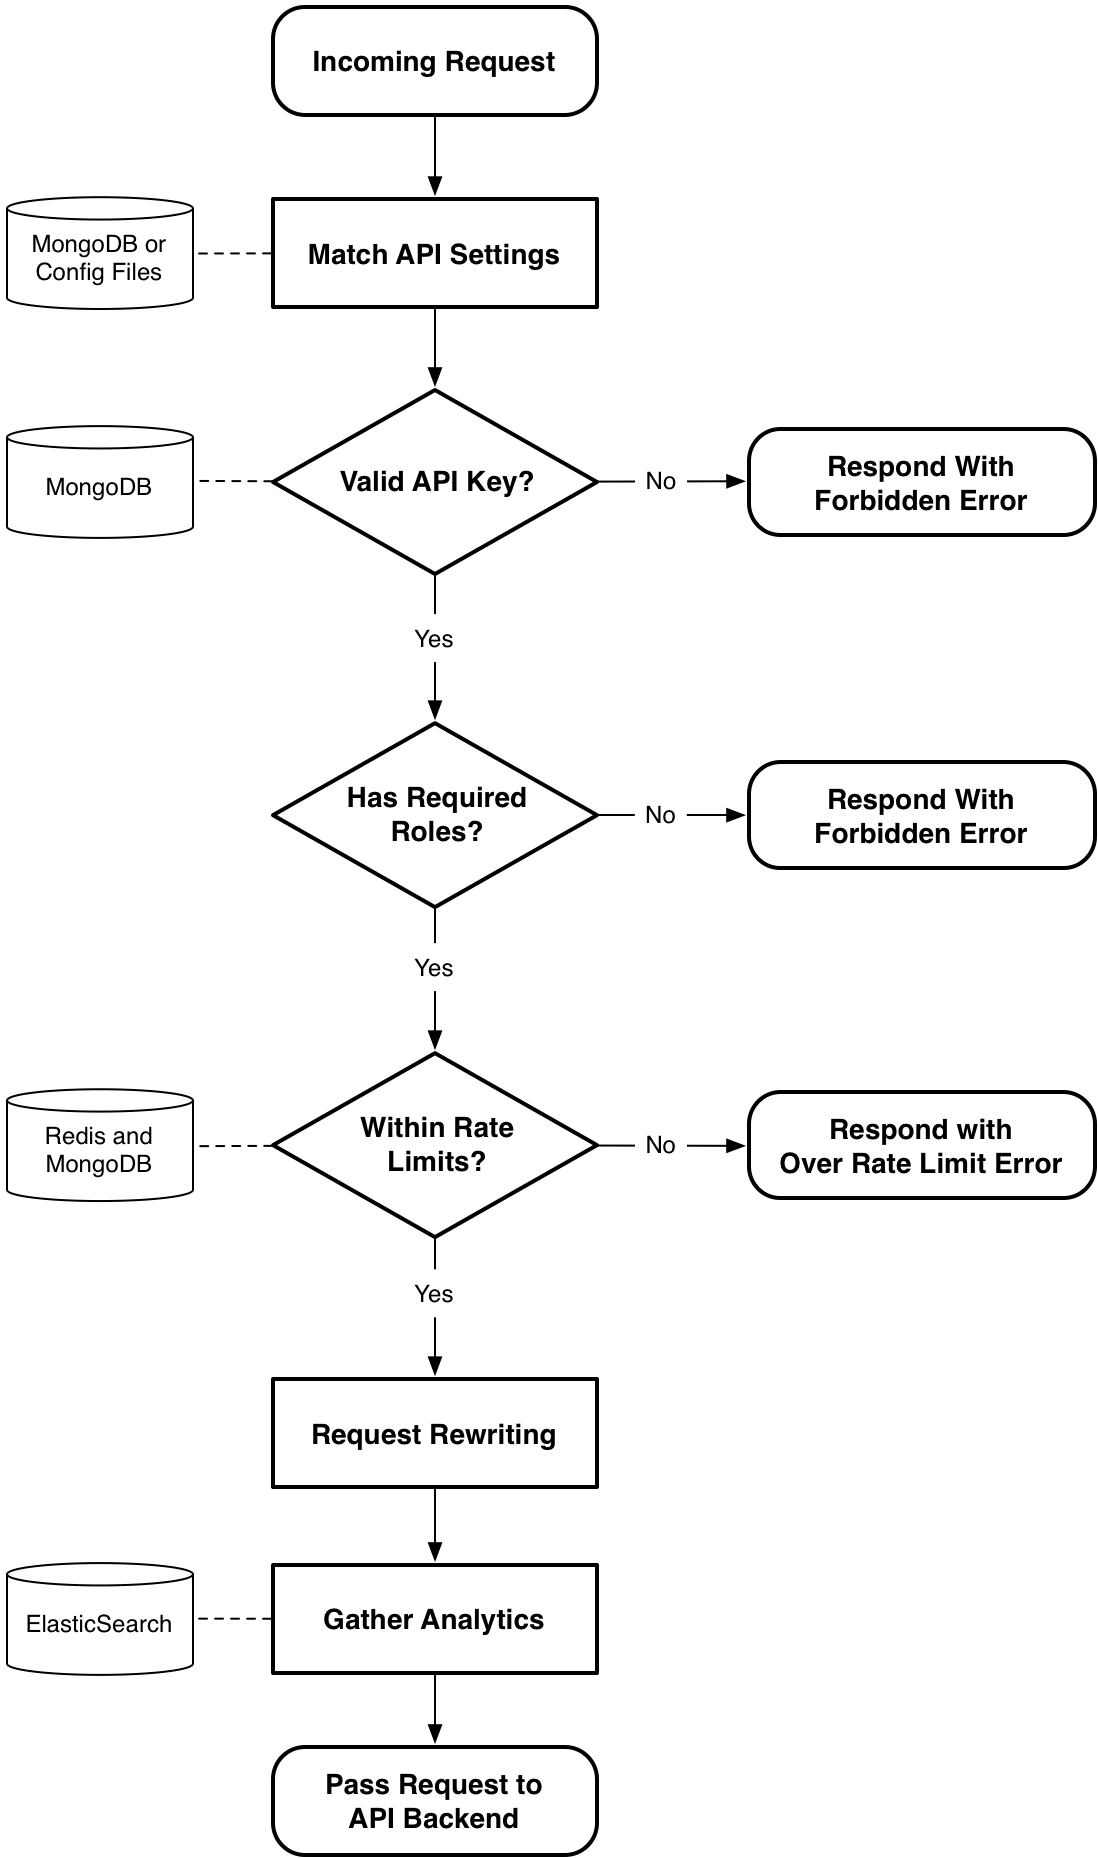
\includegraphics[width=\linewidth]{src/images/03-capitulo-3/tecnologias/api-umbrella/api-umbrella-gatekeeper.png}
  \caption{Lógica de decisión del \eng{Gatekeeper} de API Umbrella}
  \label{fig:api-umbrella-gatekeeper}
\end{figure}

\subparagraph{Instalación y prueba}

Al igual que en el caso de \nameref{soa:tecnologias:kong}, y ya que NREL provee una imagen oficial para ejecutar API Umbrella, utilizamos Docker para realizar una prueba de concepto del producto. A continuación detallamos los pasos realizados.

\begin{listing}[H]
  \bashfile{src/03-capitulo-3/tecnologias/nodo-central/code/api-umbrella/00-preparacion.sh}
  \caption{Preparación y arranque de API Umbrella}
  \label{soa:tecnologias:api-umbrella:bash-preparacion}
\end{listing}

Una vez ejecutados los comandos anteriores, tendremos una instancia de API Umbrella en ejecución en el equipo local que podrá ser accedida desde los puertos \texttt{80} y \texttt{443} de \url{localhost}. Adicionalmente al planteo que \nameref{soa:tecnologias:kong} hace con respecto a la forma de administrar el producto mediante el uso de servicios de gestión, API Umbrella también utiliza un archivo de configuración en formato \gls{lang:yaml} que puede resultar más conveniente para poder utilizar un sistema de control de versiones para versionar su contenido, pero que también implica replicarlo en cada instancia del producto que querramos ejecutar.

En el archivo de configuración debemos mínimamente definir las direcciones de correo de los usuarios que podrán acceder a la interfaz web de administración que API Umbrella provee en \url{https://localhost/admin}. Una vez identificados con alguna de esas cuentas de usuario, podremos proceder a utilizar la interfaz web para agregar una \gls{acro:api} para que API Umbrella haga de proxy de la misma. Siguiendo el ejemplo de la documentación del producto, agregamos la \gls{acro:api} de geocodificación de Google, indicando el \eng{\gls{acro:api} backend} con la dirección del servicio provisto por Google y el prefijo de las \glspl{acro:url} que nuestra instancia asociará a dicho servicio (utilizamos \texttt{/google/}), como puede observarse en la \autoref{fig:api-umbrella-api-backend}. Luego de dar de alta esta información, publicamos los cambios mediante la interfaz web y así dejamos públicamente disponible el servicio de geocodificación en nuestra instancia de API Umbrella mediante el prefijo de \gls{acro:url} \url{http://localhost/google/}.

\begin{figure}
  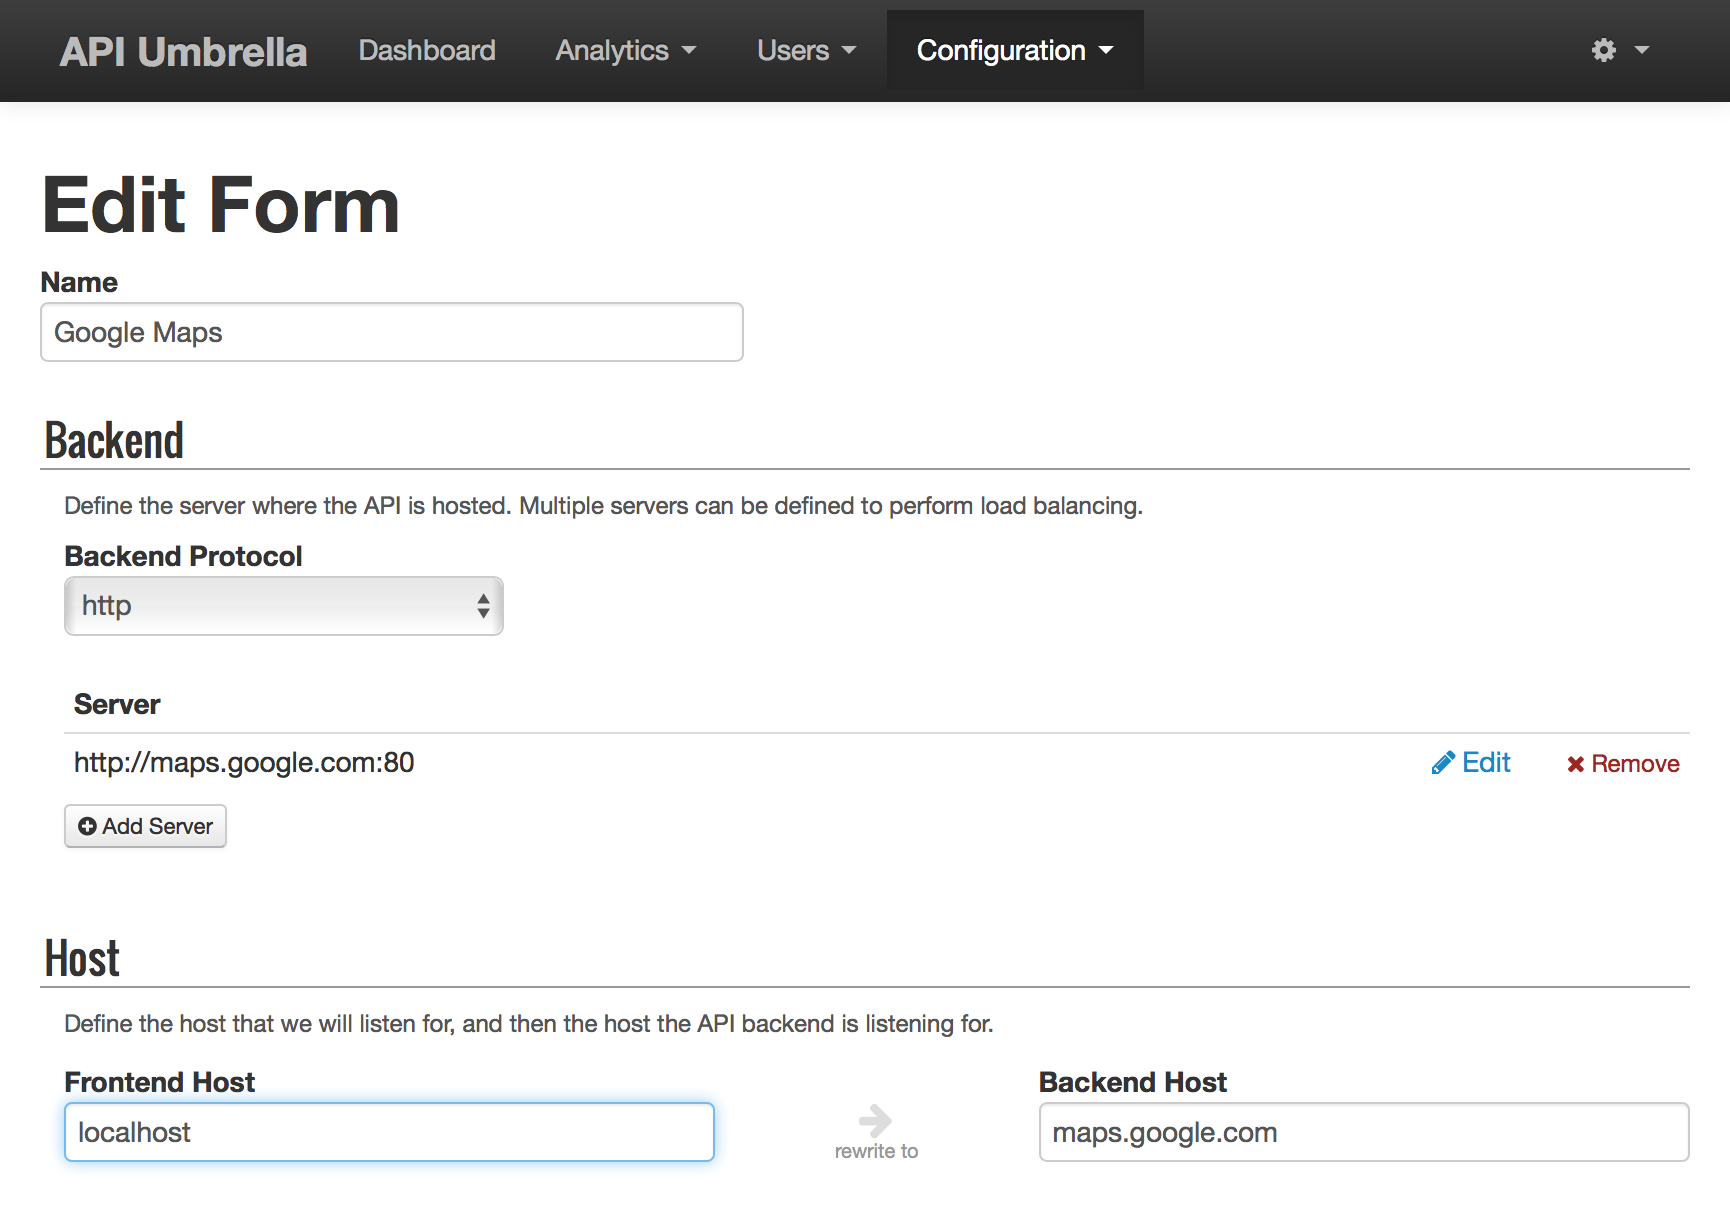
\includegraphics[width=\linewidth]{src/images/03-capitulo-3/tecnologias/api-umbrella/api-backend.png}
  \caption{Interfaz web de carga de un \eng{backend} de servicios de API Umbrella}
  \label{fig:api-umbrella-api-backend}
\end{figure}

\begin{figure}
  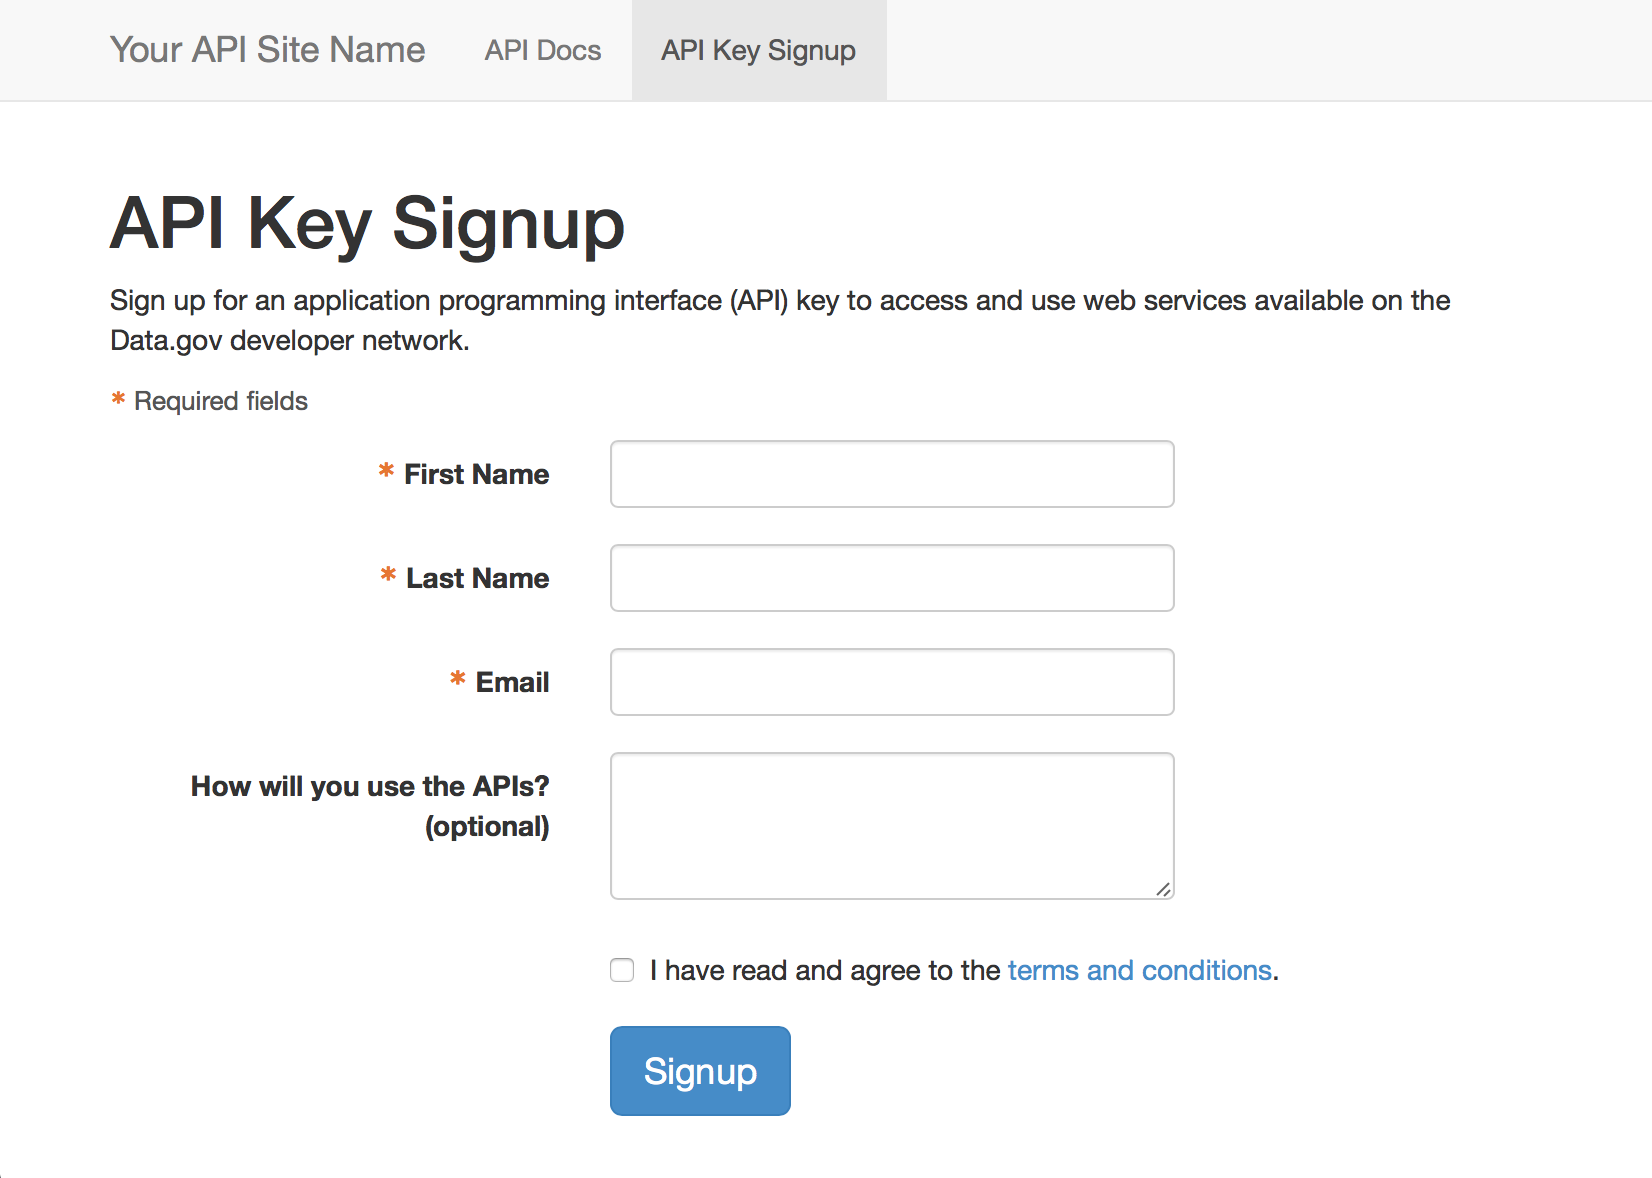
\includegraphics[width=\linewidth]{src/images/03-capitulo-3/tecnologias/api-umbrella/api-key-request.png}
  \caption{Interfaz web de solicitud de clave de acceso a los servicios de API Umbrella}
  \label{fig:api-umbrella-api-key-request}
\end{figure}

Para poder utilizar este nuevo \gls{term:endpoint} debemos obtener una clave de acceso (\eng{\gls{acro:api} key}), y para esto API Umbrella provee una interfaz web dedicada que puede observarse en la \autoref{fig:api-umbrella-api-key-request}. Completando los datos solicitados obtendremos nuestra clave de acceso para que nuestras peticiones sean autorizadas, en nuestro caso obtuvimos la clave \texttt{6dn6iL7xTuR1bvSWdRccpP7DCFp5X2OnhdYZzkrI}. Utilizando esta clave y la \gls{acro:url} definida anteriormente, podemos realizar las siguientes peticiones para probar el correcto funcionamiento del producto:

\begin{listing}[H]
  \bashfile{src/03-capitulo-3/tecnologias/nodo-central/code/api-umbrella/01-pruebas.sh}
  \caption{Prueba de uso de API Umbrella}
  \label{soa:tecnologias:api-umbrella:bash-pruebas}
\end{listing}

Con estos comandos pudimos comprobar varias situaciones:

\begin{itemize}
  \item En primer lugar, que API Umbrella requiere por defecto el uso de claves de acceso para responder a los servicios para los que funciona de proxy. Este enfoque ``seguro por defecto'' es altamente deseable, ya que implica que para consumir la información que nuestros servicios proveen, se debe obtener una clave de acceso y por ende se debe identificar al \eng{consumer} de la información - en nuestro caso, serían las aplicaciones cliente las que identifiquemos, pero si llegásemos a proveer nuestra información a terceros, éstos deberían primero identificarse para obtener una clave de acceso y así permitirnos tener una noción de quién y cuánto utiliza nuestra información.
  \item En segundo lugar, que efectivamente hay un \nameref{soa:tecnologias:varnish} funcionando internamente a API Umbrella. Esto se hace evidente en las cabeceras que esta cache compartida agrega a las respuestas \gls{proto:http}: \texttt{X-Cache} y \texttt{Age}. Adicionalmente, API Umbrella agrega las cabeceras correspondientes para indicar cuándo y por cuánto tiempo se pueden almacenar en caches intermedias las respuestas, mediante \texttt{Cache-Control} y \texttt{Expires}.
  \item También comprobamos que las respuestas tienen límites en la tasa de consultas que podemos hacer. Esto se hace evidente en las cabeceras \texttt{X-RateLimit-Limit} y \texttt{X-RateLimit-Remaining} que indican respectivamente el límite aplicable y la cantidad de peticiones que nos quedan disponibles hasta que se cumpla el período de tiempo del límite y esos contadores se reinicien.
  \item Y por último, aunque no por eso menos importante, que el producto funciona correctamente haciendo de proxy del servicio de geocodificación de Google, al devolvernos una respuesta correcta para nuestra consulta.
\end{itemize}

Luego de realizar algunas peticiones, podemos utilizar la potente herramienta de análisis de tráfico y respuestas que provee API Umbrella para tener una idea del uso que nuestra instancia está teniendo, junto con datos como quién, cuándo, cuánto, cómo y desde dónde está usando nuestras \glspl{acro:api}. En la \autoref{fig:api-umbrella-analytics} se puede apreciar, a modo de ejemplo, parte de información que se puede obtener mediante esta herramienta.

\begin{figure}
  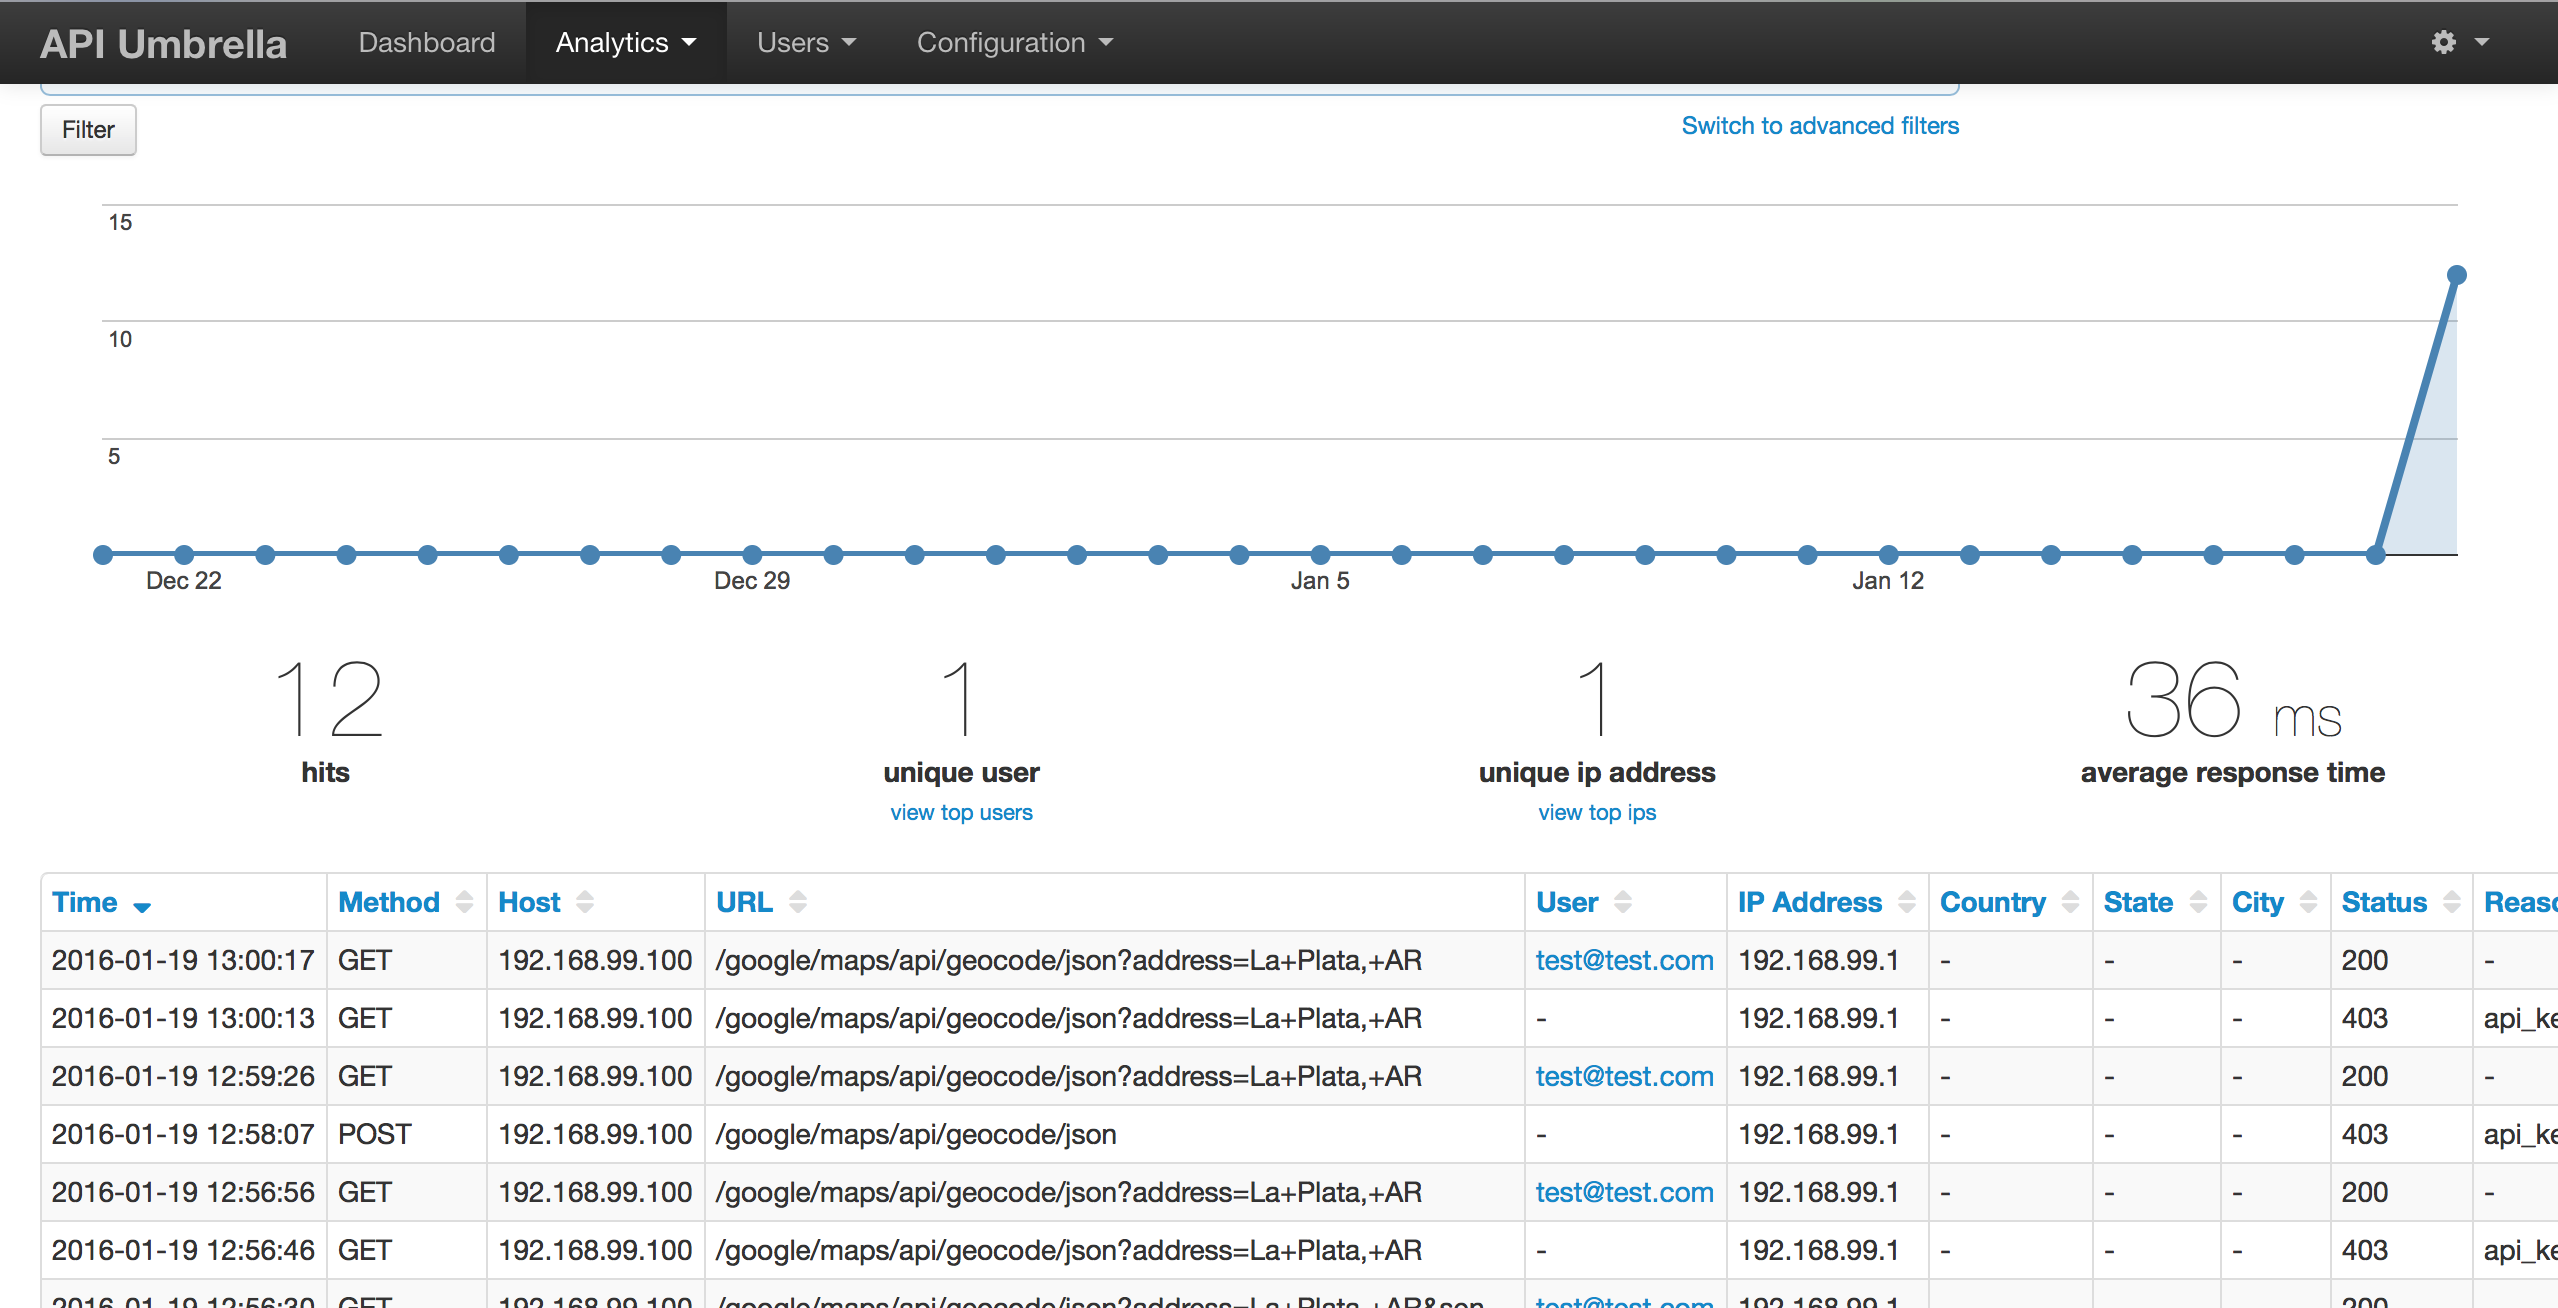
\includegraphics[width=\linewidth]{src/images/03-capitulo-3/tecnologias/api-umbrella/analytics.png}
  \caption{Interfaz web de análisis del uso de los servicios de API Umbrella}
  \label{fig:api-umbrella-analytics}
\end{figure}

\subparagraph{Madurez}

Al momento de comenzar a analizar los productos para el presente trabajo, API Umbrella se encontraba en activo desarrollo, definición y evolución. Su arquitectura interna era muy cambiante y aún le faltaban pruebas reales en ambientes productivos para poder cerrar las definiciones, por lo cual sus propios autores aconsejaban su uso únicamente para desarrollo\footnote{Hasta Diciembre de 2015, la documentación oficial del producto mostraba la leyenda ``\eng{This version is for development only}'' (``Esta versión es únicamente para desarrollo'')}.

Con la llegada de 2016 su desarrollo se desaceleró y la arquitectura quedó estabilizada, pero al momento de escritura del presente informe la herramienta carece de pruebas en producción que respalden las características que la documentación oficial describe y que nos den confianza que el producto se encuentre realmente maduro.
